\documentclass[UTF8,fontset=ubuntu]{ctexart}
\usepackage{tikz}
\usetikzlibrary{datavisualization.formats.functions}
% 1.datavisualization
% axes坐标轴,参考section 82,第872页
\begin{document}
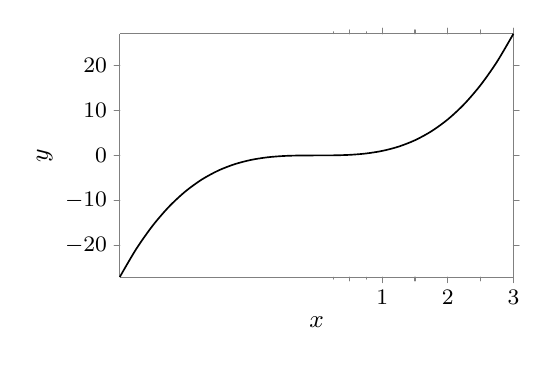
\begin{tikzpicture}
  \datavisualization [
    % 1.scientific axes,需要使用datavisualization库
    % 科学坐标轴,值格式: {<key>=<value>}可指定以下值:
    %   1)outer ticks - 刻度放置在外部
    %   2)inner ticks - 刻度放置在内部
    %   3)clean - 不在原边框画刻度,分别在左侧和下侧建立坐标轴
    %   standard labels/upright labels/end labels - 坐标标签的放置方式. 放置方式如下:
    %     [1]standard labels - x轴标签在轴中间下方;y轴标签在轴中间左侧,文字从下到上
    %     [2]upright labels - x轴标签在轴中间在下方;y轴标签在周中间左侧,文字从左到右
    %     [3]end labels - x轴标签在轴末端右侧;y轴标签在轴末端上侧,文字从左到右
    scientific axes,
    % x axis代表x轴的相关参数. 可使用参数如下:
    %   1)attribute - 轴表示的含义, 如: 时间/速度等
    %   2)label - 轴标签. 值格式为: {[<options>]<text>}
    %   3)include value - 坐标轴上必须包含的刻度. 还有类似指定最小刻度和最大刻度的关键字:
    %     [1]min value
    %     [2]max value
    %   4)logarithmic - 将数轴的刻度按指数进行递增
    %   5)length - 轴的实际长度
    %   6)unit length - 轴上步进num对应的长度, 值格式: <dimension> per <num> units
    %   7)power unit length - unit length的logarithmic版本
    %   8)ticks - 指定刻度相关. 值格式: {<key>=<value>}, key列表:
    %     [1]about - 大约指定tick个数
    %     [2]none/few/some/many - 分别代表无刻度、少量刻度(about=3)、适量刻度(about=5)、大量刻度(about=10)
    %     [3]step - 指定刻度步进
    %     [4]minor steps between steps - 大刻度之间的小刻度数量
    %     [5]major at - 详细指定大刻度的所在值, 值格式: {<list>}
    %     [6]minor at - 详细指定小刻度的所在值, 值格式: {<list>}
    %     [7]subminor at - 详细指定更小刻度的所在值, 值格式: {<list>}
    %     [8]major/minor/subminor also at - 额外附加的刻度值
    %     [9style - 对刻度线和刻度值进行配置
    %     [10]node style - 对刻度值进行配置,值格式: {<key>=<value>}. 值可以为: rotate/color等
    %     [11]tick prefix - 在刻度值前面添加的内容
    %     [12]tick suffix - 在刻度值后面添加的内容
    %     [13]tick unit - 刻度值的单位. 类似于tick suffix={$\,\rm<text>$}
    %     [14]stack - 刻度值进行错位显示(偶数项拉伸)
    %     [15]stack' - 刻度值进行错位显示(奇数项拉伸)
    x axis={label=$x$,ticks={major at={1,2,3},minor at={0.5,1.5,2.5},subminor at={0.25,0.75}}},
    y axis={label=$y$},
    % 线条类型:
    %   1)visualize as line - 直线
    %   2)visualize as smooth line - 曲线
    %   3)visualize as scatter - 描点
    visualize as smooth line]
    data [format=function] {
      var x : interval [-3:3];
      func y = \value x*\value x*\value x;
    };
\end{tikzpicture}\\\vspace{1cm}

\begin{tikzpicture}
  % 2.school book axes,需要使用datavisualization
  \datavisualization [
    school book axes,
    visualize as smooth line,
    x axis={label=$x$},
    y axis={label=$f(x)$}]
    % format=function代表使用函数,可以使用区间指定x值,需要使用datavisualization.formats.functions库
    data [format=function] {
      % x变量的取值区间
      var x : interval [-1.3:1.3];
      % y关于x的函数
      func y = \value x*\value x*\value x;
    };
\end{tikzpicture}\\\vspace{1cm}

\begin{tikzpicture}
  % 3.xy Cartesian,需要使用datavisualization
  \datavisualization [
    xy Cartesian,
    visualize as smooth line]
    data [format=function] {
      var x : interval [-1.3:1.3];
      func y = \value x*\value x*\value x;
    };
\end{tikzpicture}\\\vspace{1cm}

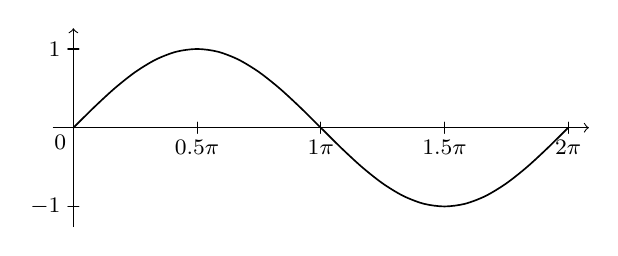
\begin{tikzpicture}
    % 作一个正弦曲线
    \def\mytypesetter#1{%
      \pgfmathparse{#1/pi}%
      \pgfmathprintnumber{\pgfmathresult}$\pi$%
    }
    \datavisualization [
    school book axes,
    x axis={ticks={step=(0.5*pi),tick typesetter/.code=\mytypesetter{##1}}},
    visualize as smooth line]
    data [format=function]{
      var x : interval [0:2*pi];
      % r用于将弧度制x转化为角度制
      func y = sin(\value x r);
    };
\end{tikzpicture}\\\vspace{2cm}


% 2.plot
\begin{tikzpicture}
    % \draw plot coordinates {<coordinate_01> <coordinate_02> ...};
    % 使用一系列坐标,进行连接作图
    \draw plot coordinates {(0,0) (1,1) (2,0)};
\end{tikzpicture}\\\vspace{1cm}
\end{document}
